%%!TEX encoding = UTF-8 Unicode
\documentclass[11pt,a4paper]{article}
\usepackage{graphicx}
\usepackage{amssymb}
\usepackage{epstopdf}
\usepackage[frenchb]{babel}
\usepackage[utf8]{inputenc}
\usepackage{listings}
\usepackage{algpseudocode}
\usepackage{algorithmicx}

\newcommand{\cad}{c'est-à-dire}

\lstdefinelanguage{Harmless}
{morekeywords={model,include,port,device,architecture,write,shared,behavior,format,select,error,warning,component,void,every,memory,width,address,type,RAM,ROM,register,stride,read,program,counter,pipeline,state,init,run,as,machine,BTB,FIFO,bypass,release,in,maps,to,stall,default,instruction,fetch,debug,big,little,endian,except,do,out,when,field,nop,slice,case,is,others,signed,or,syntax,switch,number,octal,decimal,hexadecimal,binary,suffix,prefix,timing,decode,size,jumpTaken,add,cycle,use,return,print,if,then,elseif,else,loop,while,end,true,false,ror,rol,cat,wait,for,signal,emit}, 
sensitive=true, 
morecomment=[l]{--}, 
morestring=[b]"
}

\lstset{
  basicstyle=\small,
  stringstyle=\ttfamily, % typewriter type for strings
  showstringspaces=true %space in strings
  commentstyle=\ttfamily,
 % commentstyle=\itshape\color{vert},
  identifierstyle=\ttfamily\bfseries,
  keywordstyle=\ttfamily\bfseries\underbar,
  numbers=left, numberstyle=\tiny, stepnumber=1, numbersep=5pt, %line numbers
  breaklines=true,
  frame=lines, %bottom and top lines
  language=Harmless,
  defaultdialect=Harmless,
}

%\lstset{
%  language=C,
%  basicstyle=\ttfamily\footnotesize
%}

\DeclareGraphicsRule{.tif}{png}{.png}{`convert #1 `basename #1 .tif`.png}

\title{Modélisation de la hiérarchie mémoire dans Harmless}
\author{Jean-Luc Béchennec, Mikaël Briday}
\begin{document}

\maketitle
\tableofcontents
Ce document traite de la modélisation de la hiérarchie mémoire dans le langage Harmless. Dans un premier temps, les aspects matériels de la hiérarchie mémoire sont rappelés, puis dans un deuxième temps, les concepts et éléments de modélisations dans Harmless sont exposés.

\section{Aspect matériel de la hiérarchie mémoire}

Une hiérarchie mémoire est un empilement de mémoires cache permettant un accès plus rapide aux données ou aux instructions. On a donc plusieurs niveaux de caches appelées $L_n$ ou $n$ est le niveau. Un cache est accédé de manière transparente lors du chargement des données ou des instructions. De même, sa mise à jour est faite de manière transparente.

Lorsqu'on accède à une donnée ou à une instruction, le cache du niveau courant est consulté. S'il la possède c'est un {\bf hit}, sinon c'est un {\bf miss} et la requête est adressée au niveau suivant. C'est une vision un peu naïve des choses car pour des raisons d'efficacité et d'architecture, la partie du cache permettant de savoir si une donnée est présente ou non (les {\bf tags}) peut-être placée de telle sorte qu'elle est accédé plus vite que le contenu du cache. Par exemple, les tags d'un cache $L_2$ peuvent être localisés sur la même puce que le cache $L_1$ et le processeur; dans ce cas on accède simultanément au $L_1$ et au tags du $L_2$ et en cas de miss sur le $L_1$ et de hit sur le $L_2$, lancer plus rapidement la requête au contenu du $L_2$.

Un cache possède des caractéristiques structurelles: sa {\bf taille} (en octets), son {\bf associativité} (nombre de ligne dans un ensemble), la {\bf taille de la ligne} (en octets) et le {\bf nombre d'ensembles}. Pour des raisons d'implémentation, la taille de la ligne est une puissance de 2, la taille du cache ne l'est pas nécessairement car l'associativité peut être quelconque\footnote{par exemple le cache de second niveau du processeur DEC Alpha 21164 a une associativité de 3.}.

Des caractéristiques fonctionnelles viennent s'ajouter: la {\bf politique de remplacement} lorsque l'associativité est $\geq 2$, le fait qu'il soit {\bf bloquant} ou non et le {\bf protocole de cohérence}.

Plusieurs politiques de remplacement {\it académiques} existes: FIFO, Random, NLU\footnote{Not Last Used, l'une des lignes de l'ensemble mais pas la dernière accédée.}, LRU\footnote{Least Recently Used, la ligne de l'ensemble la plus anciennement accédée}, mais les fondeurs nous en inventent une régulièrement.

Un cache bloquant est un cache qui ne peut accepter d'autre requête pendant qu'il est en train de traiter un miss. Un cache non bloquant est capable de mémoriser jusqu'à $M$ miss en cours de traitement avant de bloquer. Ce type de cache est présent dans les processeurs à ordonnancement dynamique\footnote{processeurs dits « superscalaires » et capables d'exécuter les instructions dans un ordre différent de celui spécifié dans le programme.}. On peut noter que, du fait du comportement des niveaux suivants de la hiérarchie mémoire, les requêtes peuvent ne pas terminer dans l'ordre où elles ont été lancées.

A cela, on peut ajouter la présence fréquente de tampons d'écriture en aval des caches. En effet, comme il n'y a pas de dépendance sur les écritures, on les diffère pour laisser passer les lectures. Bien évidemment, pour chaque lecture qui double une écriture, les adresses sont comparées. En cas d'égalité, on a un hit sur le tampon.

Sans entrer dans les détails, un protocole de cohérence de cache permet de synchroniser plusieurs cache afin de garantir qu'une même données présente dans plusieurs cache aura une valeur cohérente.

\section{Comment modéliser avec Harmless}

\subsection{Quelques remarques}

Tout d'abord, du fait de sa transparence, un cache ne fait pas partie de la description du jeu d'instruction. Il s'agit d'un dispositif qui doit s'insérer dans la description de la micro-architecture. Toutefois, il y a une partie fonctionnelle accessible par le jeu d'instruction lié au contrôle comme le vidage du cache (\emph{flush}) ou le blocage de certaines lignes (\emph{lock}) pour améliorer la prédictibilité.

Le cache n'intervenant pas dans les aspects fonctionnels du jeu d'instruction, il n'a pas à stocker réellement une copie des données, seule la partie permettant de savoir si une donnée ou une instruction est présente ou non est nécessaire.

Actuellement, ce qui est décrit dans la micro-architecture utilise des information issues du jeu d'instruction (classe, registres source et destination). Ce sont des informations statiques. Un cache nécessite des informations dynamiques (adresses des instructions, adresses utilisées par les instructions qui font un accès à la mémoire) et qui sont disponibles à l'exécution de l'instruction. Le plus naturel est d'espionner les accès aux {\bf components} dont on veut cacher les données.

Une façon de faire serait de pouvoir insérer le cache à l'interface du component afin de récupérer les adresses pour ensuite simuler le cache dans l'exécution temporelle.

\subsection{Modélisation du cache}

\subsection{Components}
Actuellement, les components ressemblent énormément à des classes mais ne fournissent pas la souplesse des classes des langages à objets. Il faut différencier la déclaration et l'instantiation.

Lors de la modélisation de l'ISA, on va faire un appel à un composant dans les \emph{behavior}. Par exemple, on fait un accès à l'addition de l'ALU. Cet appel ne fait pas d'hypothèse sur la micro-architecture, et ne fait pas référence à une instance particulière de l'ALU. Ainsi, par exemple, sur une architecture possédant 2 ALUs, l'instruction ne précise pas laquelle il faut utiliser (heureusement).
Ainsi, le composant fait référence à la \emph{déclaration} de l'ALU, mais pas à son instantiation.

Au niveau de la micro-architecture, il est indispensable de faire référence et l'instance de l'ALU, ceci est fait en utilisant les \emph{device}. Dans le cas d'une architecture avec 2 ALUs, dont une qui ne permette pas de faire des division, nous avons la description:
\begin{lstlisting}
  device IntDev : Integer_Unit {
    port all 
  }

  device IntWithoutDiv : Integer_Unit {
      port all except div_ov_signed,
                      div_ov_signed_withUpdateStatus,
                      div_ov_unsigned,
                      div_ov_unsigned_withUpdateStatus
  }
\end{lstlisting}

Ainsi, un \emph{component est la déclaration} et le \emph{device est l'instantiation}. Il y a toutefois une exception avec le composant mémoire, qui contient "réellement" la mémoire...
 
\subsection{Modélisation}
La modélisation du comportement temporel de la mémoire se fait à travers des automates temporisés qui se synchronisent sur des \emph{signaux} (équivalent aux \emph{channel} de \emph{Uppaal}). Ainsi, chaque élément de la hiérarchie mémoire (mémoire centrale, et les différents niveaux de cache) se compose de:
\begin{itemize}
\item Un \emph{composant} qui modélise la partie fonctionnelle de l'élément (cache, mémoire). On va intégrer ici la partie algorithmique du cache (comment est implémenté la politique de remplacement, l'associativité, ...);
\item Un \emph{device} qui va représenter l'instance de l'élément.
\item Une partie \emph{timing} qui va implémenter la synchronisation temporelle de l'élément à travers une représentation textuelle d'un automate temporisé. Cette partie timing va notamment pouvoir se synchroniser sur des signaux avec les niveaux inférieurs et supérieurs de la hiérarchie mémoire, ainsi que faire des attentes.
\end{itemize}
Ces 3 éléments sont décrits dans la suite du document.
Enfin, une dernière partie permet de connecter les signaux entre les instances des différents niveaux de la hiérarchie mémoire.

\subsection{Implémentation fonctionnelle du cache}
La partie fonctionnelle est décrite dans un \emph{composant}. Les ajouts à réaliser par rapport à la version actuelle concernent essentiellement la possibilité de gérer des tableaux et des types de données structurés.
Les structures se définissent en utilisant le mot clé \texttt{type}:
\begin{lstlisting}
  type cacheLine {
    u24  tag
    u1   valid
  }
\end{lstlisting}
Les tableaux sont définis entre crochets, mais contrairement en C, les crochets sont du côté du type:
\begin{lstlisting}
  type cacheSegment {
    cacheLine[64] lines
  }
\end{lstlisting}
Ce sont les seules différences à apporter sur les composants. Ainsi, pour le modèle du cache d'instruction de l'ARM9, les fonctions suivantes sont implémentées.
\begin{lstlisting}
  u1 isInCache(u24 tag,u3 seg)       -- presence en cache
  void reset()                       -- init
  void insertInCache(u24 tag,u3 seg) -- insertion
  u1 readAccess(u32 addr)            -- acces complet
\end{lstlisting}
C'est un modèle partiel, on pourrait notamment rajouter ici toutes les fonctions qui permettent de configurer le cache.

\subsection{Instanciation}
L'instantiation se fait à travers un \emph{device}, de manière classique dans la section \emph{architecture}:
\begin{lstlisting}
device DevICacheARM920T : ICacheARM920T {}
\end{lstlisting}
On peut bien sûr imaginer intégrer des ports pour intégrer des contraintes pour les instructions qui accèdent à la configuration du cache.

\subsection{Synchronisation}
La synchronisation entre les différents niveaux de cache à travers une modélisation interne sous forme d'automate temporisé. Une section \emph{timing} est utilisée. 

Dans une section timing, on peux se synchroniser avec d'autres automates (qui modélisent les niveaux hiérarchiques de mémorisation supérieurs ou inférieurs) à travers des signaux. Quand il y a \emph{émission} d'un signal, il y a une synchronisation avec le \emph{récepteur}: \emph{À la fois l'émission et la réception sont bloquants} (comme dans les \emph{channels} de Uppaal). L'objectif est de pouvoir dans un 2e temps s'interfacer avec Uppaal pour effectuer du modèle checking (liveness, deadlock, ...).

Les éléments remarquables sont:
\begin{itemize}
\item l'émission d'un signal: \texttt{emit signal icacheEnd}
\item l'attente d'un signal: \texttt{wait for signal icacheEnd}
\item l'attente d'un certain temps: \texttt{wait \textit{n} cycle}
\item des boucles: \texttt{loop 3 while(nb < 4) .. end loop}, où le \texttt{3} correspond à la guarde (le nombre maximal de tours de boucle).. \texttt{TODO: Trop expressif => pas facilement simplifiable?} Est-ce que mettre une structure plus contrainte comme \texttt{do \textit{3} times ... end do} où le paramètre de boucle est une constante et non pas une expression.
\end{itemize}

Soit par exemple la modélisation d'une mémoire avec un \textsl{burst}: On mets \textit{m} cycles pour avoir la première donnée, puis ensuite il suffit de \textit{n} cycle pour avoir les 3 données suivantes. La représentation sous forme d'automate peut-être la suivante:

\begin{figure}[htbp] %  figure placement: here, top, bottom, or page
   \centering
   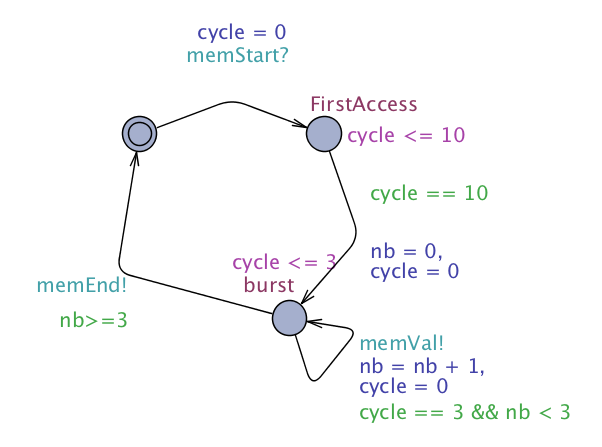
\includegraphics[width=0.5 \linewidth]{memBurstUppaal.png} 
   \caption{Modélisation de la mémoire (burst) en Uppaal. \texttt{cycle} est une horloge. On trouve sur les transitions : les \emph{gardes} en vert (condition de passage), les \emph{mise à jour} en bleu (action à réaliser quand la transition est prise), les \emph{synchronisations} en bleu clair  (! émission, ? réception). On trouve sur les places: l'\emph{invariant} en violet et le \emph{nom} de la place en rouge.}
   \label{fig:automateMem}
\end{figure}

Sa représentation textuelle en Harmless deviendrait alors:
\begin{lstlisting}
timing mem
  signal in : memStart
  signal out: memEnd, memVal
{
  u3 nb
  wait for signal memStart
  wait 10 cycle
  emit signal memVal
  nb := 0
  loop 3
  while(nb < 3)
    wait 3 cycle 
    emit signal memVal
    nb := nb+1
  end loop
  emit signal memEnd
}
\end{lstlisting}

La section \texttt{timing} n'est pas incluse dans une section \texttt{architecture}.

\subsection{Assemblage du tout}
\label{sec:assemblage}
L'assemblage consiste à connecter les signaux (\emph{un} émetteur avec \emph{un} récepteur) afin de modéliser le tout. On trouve une section \emph{signal} dans la section \emph{architecture}. On fait toujours référence à un signal \emph{d'un device}.
La connexion entre le cache d'instruction et la mémoire centrale peut s'exprimer comme ceci:
\begin{lstlisting}
  --connect cache to main memory
  DevICacheARM920T.memStart  -> MemDev.memStart
  MemDev.memEnd              -> DevICacheARM920T.memEnd
  MemDev.memVal              -> *                       --not connected
\end{lstlisting}
Dans cet exemple, le \emph{device} \texttt{MemDev} modélise la mémoire, et \emph{DevICacheARM920T} est le \emph{device}du cache d'instruction.

D'autre part, il faut aussi connecter l'accès à la mémoire (qui est fait à travers le composant mémoire par les instructions) et la mémoire cache. On fait ici encore référence au \emph{device}. En effet, le \emph{device} associé à la mémoire est:
 \begin{lstlisting}
device MemDev : mem {
  read is ram_read8 | ram_read16 | ram_read32 
  write is ram_write8 | ram_write16 | ram_write32
  shared port fetch : read
  shared port loadStore : read or write
}
\end{lstlisting}
Ainsi, un signal peut-être associé à un \emph{port partagé}. Ici, ce sera le port \emph{fetch} pour le cache d'instruction. Un accès en lecture renverra sur le port \emph{fetch} ou le port \emph{loadStore} et donc le cache d'instruction ou de données.
 \begin{lstlisting}
  -- il faut mettre que c'est le fetch, car suivant le port, 
  -- on ne fait pas reference au meme cache (instruction, data).
  -- le port doit etre shared (generation du controleur)
  MemDev.fetch(addr) -> DevICacheARM920T.iCacheStart(addr) until DevICacheARM920T.icacheEnd
\end{lstlisting}

Un exemple dans le fichier memoireCache.hadl.
\section{Modélisation interne sous forme d'automate temporisé}
Lors de la description de la partie \emph{timing}, l'analyse syntaxique est accompagnée d'une analyse sémantique qui se contente de remplir les structures de données des \emph{timingInstructions} : émission d'un signal, réception d'un signal, attente d'un signal ou d'une expression, boucles, ..
Il faut ensuite faire un traitement permettant de remplir les structures de données représentant l'automate temporisé: \emph{timingAutomata}, \emph{timingAutomataPlace}, \emph{timingAutomataTransition}. Dans une \emph{timingAutomataTransition}, nous avons:
\begin{itemize}
\item une liste de \emph{mise à jour} (\emph{update}): action associée à la transition;
\item une liste de \emph{garde} (\emph{guard}): condition de passage de la transition;
\item une liste de \emph{synchronisation}: envoi ou réception de signaux (bloquants en réception/émission, comme Uppaal);
\end{itemize}
Dans une place, il y a:
\begin{itemize}
\item un nom;
\item une liste \emph{d'invariants}: conditions qui restent valables tant qu'on est dans la place.
\end{itemize}

L'objectif est d'avoir à la fois un export vers l'outil de model checking \emph{Uppaal} pour permettre de vérifier qu'il n'y a pas d'interblocage (deadlock) entre les différents automates modélisés, mais aussi bien sûr d'avoir un modèle de simulation (figure \ref{fig:automateFlotConstruction}).
\begin{figure}[htbp] %  figure placement: here, top, bottom, or page
   \centering
   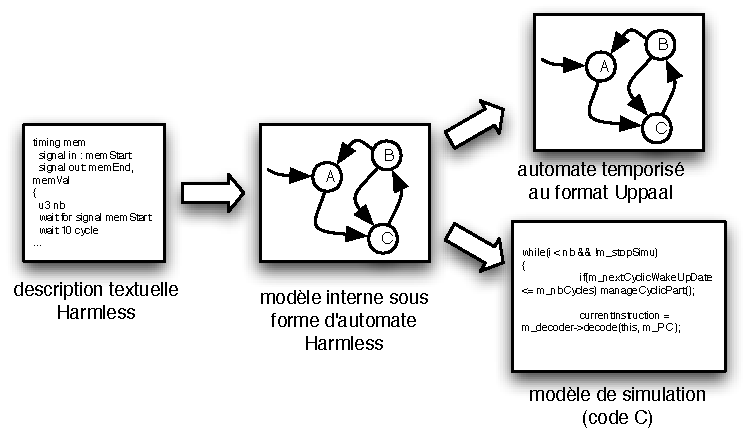
\includegraphics[width=\linewidth]{automateFlotConstruction.pdf} 
   \caption{Flot de construction de l'automate.}
   \label{fig:automateFlotConstruction}
\end{figure}
À partir de la description, un modèle intermédiaire qui est l'automate temporisé \emph{Harmless} est généré. Celui-ci a des informations de haut niveau qui seront ensuite utilisées pour générer à la fois l'automate temporisé avec la sémantique d'Uppaal, et à la fois le code permettant la simulation du modèle d'automate. 

La génération du modèle de simulation n'est pas directement déduite du modèle temporisé au format Uppaal pour des raisons d'efficacité. En effet, la  différence se situe au niveau de la gestion du temps. La commande \emph{Harmless} \texttt{wait xx cycle} permet de faire une attente de plusieurs cycles. Il n'existe pas de primitive de haut niveau dans Uppaal permettant de faire cette modélisation, et il est alors nécessaire d'utiliser une horloge.

\begin{figure}[htbp] %  figure placement: here, top, bottom, or page
   \centering
   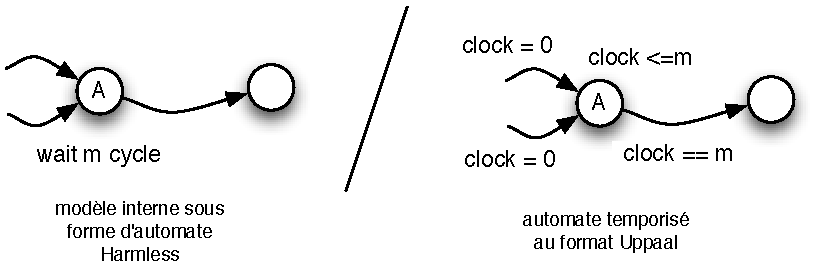
\includegraphics[width=\linewidth]{automateWaitCycleDiff.pdf} 
   \caption{Différence entre l'automate Harmless et Uppaal}
   \label{fig:automateWaitCycleDiff}
\end{figure}

Dans le schéma \ref{fig:automateWaitCycleDiff}, la commande \emph{Harmless} (\texttt{wait xx cycle}) est modélisée sous la forme d'une attente lié à l'état A. Dans la modélisation \emph{Uppaal}, on utilise une horloge qui est initialisée lors des transitions vers l'état A, puis on utilise une condition sur les transitions de sortie et un invariant sur l'état (pas forcément indispensable).

En utilisant directement l'approche d'Uppaal, il serait nécessaire de vérifier l'état de la condition à chaque cycle de la simulation, ce qui n'est pas efficace en terme de vitesse de simulation. Par contre, l'utilisation d'une primitive de haut niveau d'attente au niveau du modèle de simulation permet de suspendre l'activité de l'automate pendant la durée d'attente. Il est à noté que sur la modélisation de la hiérarchie mémoire, ces temps d'attente peuvent être long (plusieurs centaines de cycles lors d'un accès à la mémoire centrale).

\appendix
\section{Génération des structures de données de l'automate Harmless à partir de la description textuelle}
Cette section permet de décrire les règles de génération de l'automate Harmless à partir de la description textuelle. Chaque instruction Harmless est associée à un patron (\emph{pattern}) d'automate. Les règles sont ici présentées à partir d'un état courant A.

\subsubsection{init}
À l'initialisation, il ne devrait y avoir qu'un seul état vide. Cependant, certaines instructions Harmless requièrent l'accès au transitions qui arrivent sur l'état courant. Ces transitions qui arrivent s'ur l'état initial ne sont connues qu'à la fin de la construction (quand on reboucle). Par commodité, et sans changer la sémantique, 2 états sont ajoutés à l'initialisation:

\begin{figure}[htbp] %  figure placement: here, top, bottom, or page
   \centering
   \includegraphics[width=0.3 \linewidth]{automateInit.pdf} 
   \caption{Initialisation du système avec 2 états, pour que les transitions qui arrivent sur l'\emph{état courant} de la prochaine instruction soient connues.}
   \label{fig:automateInit}
\end{figure}



\subsubsection{wait for signal}
L'instruction d'attente d'un signal (\emph{wait for signal memStart}) provoque:
\begin{itemize}
\item l'ajout d'une transition, avec la réception de \emph{memStart} dans la partie \emph{synchronisation} de la transition. On crée alors une nouvelle place;
\end{itemize}

\begin{figure}[htbp] %  figure placement: here, top, bottom, or page
   \centering
   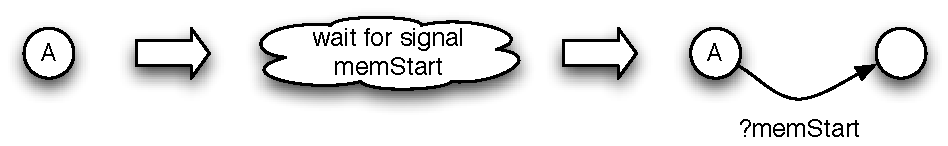
\includegraphics[width=\linewidth]{automateWaitForSignal.pdf} 
   \caption{\emph{Timing instruction} relative à \emph{wait for signal memStart}}
   \label{fig:automateWaitForSignal}
\end{figure}

\subsubsection{emit signal}
De même l'instruction d'émission d'un signal (\emph{emit signal memVal}), provoque:
\begin{itemize}
\item l'ajout d'une transition, avec l'émission de \emph{memVal} dans la partie \emph{synchronisation} de la transition. On crée alors une nouvelle place;
\end{itemize}

\begin{figure}[htbp] %  figure placement: here, top, bottom, or page
   \centering
   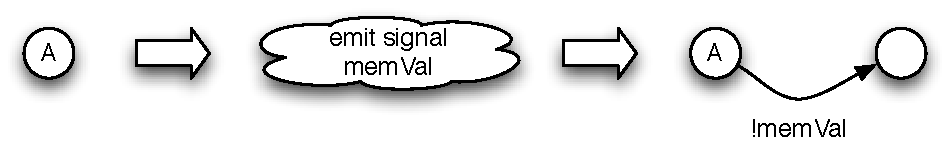
\includegraphics[width=\linewidth]{automateEmitSignal.pdf} 
   \caption{\emph{Timing instruction} relative à \emph{emit signal memVal}}
   \label{fig:automateEmitSignal}
\end{figure}

\subsubsection{wait m cycle}
L'attente d'un certain nombre de cycle est associé à un état de l'automate Harmless. S'il y avait dans l'instruction précédente une autre attente, les 2 attentes sont simplement ajoutées.

\begin{figure}[htbp] %  figure placement: here, top, bottom, or page
   \centering
   \includegraphics[width=\linewidth]{automateWaitCycleHarmless.pdf} 
   \caption{\emph{Timing instruction} relative à \emph{wait m cycle}}
   \label{fig:automateWaitCycle}
\end{figure}

%L'attente d'un certain nombre de cycle requiert l'utilisation d'une \emph{horloge}. Toutes les horloges sont initialisées à 0 au démarrage. L'instruction \emph{wait m cycle} provoque:
%\begin{itemize}
%\item la création d'une horloge: à rajouter dans une liste des horloges pour l'automate.
%\item l'ajout de l'initialisation de l'horloge dans toutes les places qui arrivent sur la place courante
%\item l'ajout d'un invariant sur la place courante: \emph{horloge < m}
%\item l'ajout d'une transition (et création d'un nouvel état courant) avec la garde: \emph{horloge == m}.
%\end{itemize}
%
%\emph{Note:} lors de la création de l'automate, on connait forcément toutes les transitions qui pointent vers une place de l'automate. Le modèle de l'état initial le permet.
%
%\begin{figure}[htbp] %  figure placement: here, top, bottom, or page
%   \centering
%   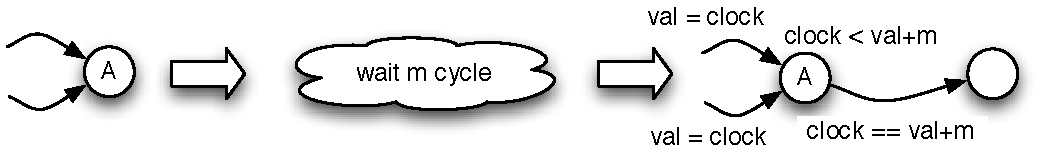
\includegraphics[width=\linewidth]{automateWaitCycle.pdf} 
%   \caption{\emph{Timing instruction} relative à \emph{wait m cycle}}
%   \label{fig:automateWaitCycle}
%\end{figure}

\subsubsection{affectation}
L'affectation implique la création d'un nouvel état, comme dans le schéma:

\begin{figure}[htbp] %  figure placement: here, top, bottom, or page
   \centering
   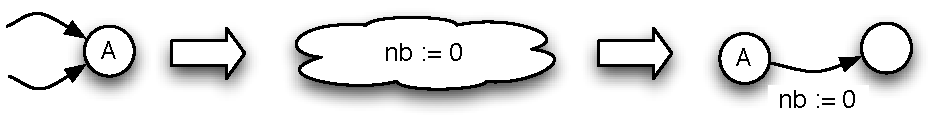
\includegraphics[width=\linewidth]{automateAffectation.pdf} 
   \caption{\emph{Timing instruction} relative à l'affectation}
   \label{fig:automateAffectation}
\end{figure}

\subsubsection{la boucle}

La boucle (loop \emph{max} while(\emph{$<$exp$>$}) \emph{$<$timingInstList$>$} end loop) est la plus complexe. On doit gérer une variable de boucle pour s'assurer de ne pas faire plus que \emph{max} tours (\emph{i} dans le dessin):
\begin{itemize}
\item sur la place courante (A), on teste que l'index ne dépasse pas le nombre maxi de tours: $i < max$
\item ajout d'une transition avec garde sur la transition (test si $<$exp$>$ vraie). On crée une nouvelle place (B) qui sert de point de départ pour la liste des instructions du corps de la boucle.
\item une fois les instructions du corps de la boucle terminées, on ajoute une transition, avec incrémentation de la variable de boucle dans \emph{update}
\item ajout d'une transition avec garde sur la transition (test si $<$exp$>$ fausse). On crée une nouvelle place (C) qui sert de point de sortie de la boucle.
\end{itemize}

\begin{figure}[htbp] %  figure placement: here, top, bottom, or page
   \centering
   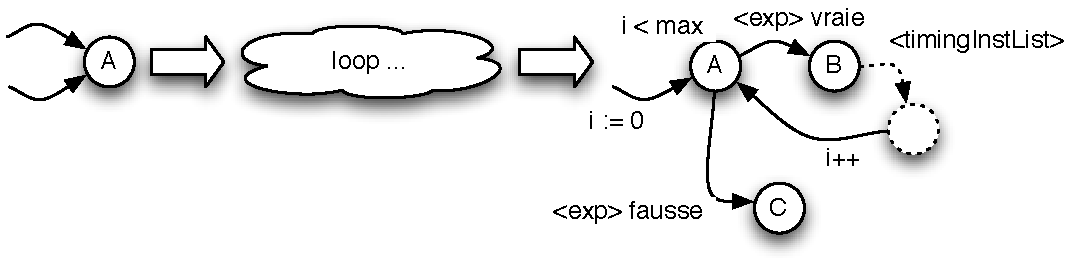
\includegraphics[width=\linewidth]{automateLoop.pdf} 
   \caption{\emph{Timing instruction} relative à l'affectation}
   \label{fig:automateLoop}
\end{figure}

\subsubsection{fin}
À la fin de la liste des instructions, on fait une transition sur la place init pour recommencer un autre cycle.

\section{Moteur de simulation}
Cette section explique comment est implémenté l'automate de simulation dans le simulateur Harmless.
La simulation du simulateur en mode CAS (\emph{Cycle Accurate Simulation}) consiste à avoir une méthode permettant de simplement simuler l'avancement d'un cycle dans le pipeline. Le simulateur va simplement faire avancer le modèle de l'automate d'un cycle, puis gérer les notifications reçues par le modèle (les notifications indiquent la présence d'un accès mémoire, de la sortie d'une instruction du pipeline, donne des informations pour la gestion des dépendances de données, ...). De plus, cette fonction indique si une instruction est sortie du pipeline:

\lstset{language=C}
\begin{lstlisting}
bool arch::execOneCycle()
{
	const unsigned int notification = m_pipeline-> execOneState(..);
	//gestion des notifications envoyees...
	m_nbCycles++;
	return instExecuted;
}
\end{lstlisting}

\subsection{Contraintes}
Ce modèle doit être étendu pour permettre la simulation de tous les automates modélisant la gestion mémoire. Il y a 2 contraintes très fortes liées à la simulation.

La première difficulté consiste à avoir un code particulièrement efficace en temps de traitement car la fonction assurant la simulation d'un cycle d'horloge est appelée très souvent (plusieurs dizaines de millions de fois par seconde). Par conséquent, la simulation de ces automates devra permettre de désactiver temporairement les automates qui sont soit en attente d'un évènement (rendez-vous), soit en attente d'un certain nombre de cycles.

Une autre contrainte est lié à la nature séquentielle de la simulation, alors que les automates évoluent naturellement en parallèle. La gestion par le moteur de simulation devra séquentialiser l'exécution des automates tout en gardant la même sémantique que le comportement en parallèle.

Un des avantage de la simulation réside dans le fait que le temps simulé peut-être arrêté suffisamment longtemps pour permettre de mettre à jour tous les états.

\subsection{Choix techniques sur l'avancement de la simulation}

L'avancement des automates associés à la gestion de la mémoire sont guidés par le temps (\texttt{wait xx cycle}), mais aussi par les évènements (\texttt{wait for signal yy}, \texttt{emit signal zz}). 

La synchronisation se fait par un rendez-vous: association entre le \emph{emit signal} d'un automate et le \emph{wait for signal} d'un autre automate. Lorsqu'un rendez-vous est possible, il sera pris en compte au plus tôt, \cad\ dès que le $2^{e}$ automate vient faire le test sur la présence du signal. Cette synchronisation est appelée synchronisation urgente dans Uppaal.

Les synchronisations impliquent un seul producteur et un seul consommateur. Ceci permet des simplifications dans les structures de données et le traitement lié à la synchronisation. Pour les exemples liés à la hiérarchie mémoire que nous avons traité, cette limitation ne semble pas gênante. Elle pourra être levé si nécessaire (au prix d'un traitement plus lent).

Les attentes pour 2 signaux ne sont pas non plus prises en compte. Actuellement, ce n'est pas possible au niveau de la description textuelle en entrée. Il pourra être envisagé si nécessaire de rajouter les attentes de plusieurs signaux (\texttt{wait for signal sig1 or sig3} par exemple).

L'automate en cours de simulation avancera au plus loin possible, jusqu'à un blocage (synchronisation ou attente de cycles). Ceci implique que dans la modélisation d'un automate, il y ait au moins une synchronisation ou une attente de cycle. Dans le cas contraire, la simulation de l'automate partirait dans une boucle infinie. Ce point est vérifié lors de la compilation par Harmless.

\subsection{Mise en œuvre de l'attente de cycles}
Un automate fait une attente pour un certain nombre de cycles à travers l'instruction \texttt{wait for xx cycle}. Pour des raisons de performances, il n'est pas envisageable de faire un test à chaque cycle pour vérifier si l'attente est terminée (attente active).

Pour l'implémentation, nous utilisons une liste chainée triée dans l'ordre croissant des dates de réveil (absolu). Le premier élément de la liste nous permet de déterminer quel est la date de prochain réveil. Par conséquent, il est nécessaire de faire seulement un test pour l'ensemble des automates en attentes. 

\subsection{Mise en œuvre de la synchronisation}
La synchronisation est basée sur un rendez-vous. Ceci implique que l'automate qui fait un \texttt{emit signal} et l'automate qui fait un \texttt{wait for signal} vont être bloqués tant qu'un seul des 2 automates est au point de rendez-vous. On va utiliser pour la simulation 2 tables statiques (générées au moment de la compilation) et 2 tables dynamiques pour la gestion en cours d'exécution. 

\subsubsection{Les tables statiques}

Les 2 tables statiques permettent de faire le lien entre le signal émis et le signal reçu. Elles sont directement liées au connexions qui sont effectuées dans la partie \texttt{signal} de la section \texttt{architecture} de la description:
\begin{lstlisting}
    --connect cache to main memory
    MemDev.memEnd              -> DevICacheARM920T.memEnd
    MemDev.memVal              -> *                       --not connected
    DevICacheARM920T.memStart  -> MemDev.memStart
\end{lstlisting}
À chaque signal est associé un index et les 2 tableaux permettent de trouver l'émetteur (\texttt{emit}) connaissant le destinataire (\texttt{wait}) ou l'inverse (figure \ref{fig:automateSynchroTabStatique}). Ces tables sont utiles pour faire les liens entre les différents éléments matériels (ici les niveaux de cache). Les signaux n'ont pas le même nom dans les différents automates (comme le fait Uppaal par exemple) pour pouvoir facilement modifier les liens entre ces éléments matériels (par exemple, ajouter un niveau de cache L2 entre le niveau L1 et la mémoire centrale, sans avoir à modifier la modélisation de L1 et de la mémoire centrale).
\begin{figure}[htbp] %  figure placement: here, top, bottom, or page
   \centering
   \includegraphics[width=0.6 \linewidth]{automateSynchroTabStatique.pdf} 
   \caption{Tableaux statiques permettant de faire les liens entre le nom du signal source et la destination. Dans cet exemple, le signal \texttt{Sig1} (index1) est envoyé et est reçu par le signal \texttt{sig3} (index 3).}
   \label{fig:automateSynchroTabStatique}
\end{figure}

\subsubsection{Les tables dynamiques}

Les 2 tables dynamiques permettent d'enregistrer les informations liées à la transition en attente, en utilisant un pointeur sur la structure qui contient l'ensemble des données liées à la transition sensibilisée. S'il n'y a aucun signal en attente, alors il y a un pointeur nul dans le tableau.

Considérons le scénario suivant: le signal \texttt{sig1} est connecté au signal \texttt{sig3}. Le premier est émis par un premier automate \texttt{A1} (\texttt{emit signal sig1}). Il est synchronisé avec l'automate \texttt{A2} qui a l'instruction \texttt{wait for signal sig3}. L'algorithme suivant est alors suivi:
\begin{itemize}
\item on récupère l'index du signal cible dans la liste statique (\texttt{signalLinksTo}). La valeur obtenue est 3, qui est l'index du signal \texttt{sig3};
\item on inspecte dans la table dynamique \texttt{signalWaitBlocked} pour savoir si le signal est en attente par l'autre automate impliqué dans la synchronisation (\texttt{A2});
\item le pointeur obtenu dans la table est nul, \cad\ que l'autre automate n'est pas encore arrivé à l'instruction \texttt{wait for signal sig3}. On insère alors dans la table dynamique  \texttt{signalEmitBlocked} le pointeur sur les données de la prochaine transition sensibilisée (figure \ref{fig:automateSynchroTabDynamique});
\end{itemize}

\begin{figure}[htbp] %  figure placement: here, top, bottom, or page
   \centering
   \includegraphics[width=0.6 \linewidth]{automateSynchroTabDynamique.pdf} 
   \caption{Tableaux dynamique permettant de gérer les synchronisations.}
   \label{fig:automateSynchroTabDynamique}
\end{figure}

À ce stade, l'automate \texttt{A1} est bloqué et le simulateur n'est pas du tout ralenti (pas de test périodique). À la date où l'automate \texttt{A2} arrive sur le point de synchronisation (\texttt{wait for signal sig3}), l'algorithme suivant est utilisé:
\begin{itemize}
\item on récupère l'index du signal source dans la liste statique (\texttt{signalLinksFrom}). La valeur obtenue est 1, qui est l'index du signal 1;
\item on inspecte dans la table dynamique \texttt{signalEmitBlocked} pour savoir si le signal est en attente par l'autre automate impliqué dans la synchronisation (\texttt{A1});
\item le pointeur obtenu dans la table est n'est pas nul cette fois car l'automate \texttt{A1} est déjà bloqué.;
\item l'automate \texttt{A1} est alors relancé car le point de rendez-vous est atteint, jusqu'à un nouveau blocage pour une attente de signal ou une attente temporelle. Le tir de la transition de l'automate et la suite de la simulation de l'automate peut entrainer des points de synchronisations avec d'autres automates qui vont eux aussi avancer dans leur exécution;
\item l'automate \texttt{A2} continue d'avancer jusqu'à un prochain point de blocage, en activant potentiellement d'autres automates suite à des points de synchronisation. Tout ceci est réalisé dans le même cycle d'horloge au niveau de la simulation. 
\end{itemize}

L'autre cas possible est symétrique est arrive si l'automate \texttt{A2} atteint le premier sur le point de synchronisation.

\subsection{Simulation: assemblage du tout}

À l'initialisation, tous les automates sont démarrés au cycle 0, avant le démarrage de la simulation. Leur comportement est simulé jusqu'au premier blocage (attente de temps ou synchronisation). La simulation commence. La seule modification au niveau de la fonction de simulation concerne la gestion de la liste chaînée associée aux attentes de cycles.

À chaque cycle, la valeur courante du nombre de cycle est comparée à la valeur en tête de liste. Si la valeur est identique, l'entrée en tête de liste est enlevée et l'automate associé est réveillé. l'automate avance alors jusqu'à un nouveau blocage (temporel/synchronisation). Ce comportement est réalisé tant que la valeur du nombre de cycle courant est égal à la date de la première entrée dans la liste chaînée (il peut bien sûr y avoir plusieurs entrées à la même date).

 \end{document}